\documentclass[tikz]{standalone}
\usetikzlibrary{calc}
\begin{document}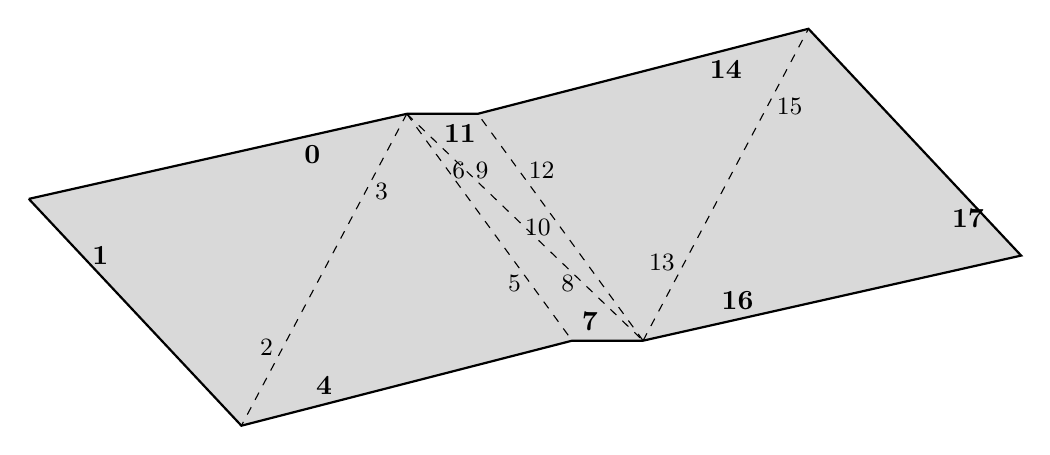
\begin{tikzpicture}[scale=0.6]
% make roughly the same picture as Yoccoz
\coordinate (zA) at (8,1.8);
\coordinate (zB) at (1.5,0);
\coordinate (zC) at (7,1.8);
\coordinate (zD) at (4.5,-4.8);

\coordinate (t0) at (0,0);
\coordinate (t1) at ($(t0)+(zA)$);
\coordinate (t2) at ($(t1)+(zB)$);
\coordinate (t3) at ($(t2)+(zC)$);
\coordinate (t4) at ($(t3)+(zD)$);


\coordinate (b0) at (0,0);
\coordinate (b1) at ($(b0)+(zD)$);
\coordinate (b2) at ($(b1)+(zC)$);
\coordinate (b3) at ($(b2)+(zB)$);
\coordinate (b4) at (t4);

\filldraw[thick,black,fill=gray!30] (t0) 
  -- node[below,near end] {\bf 0} (t1)
  -- node[below,near end] {\bf 11} (t2)
  -- node[below,near end] {\bf 14} (t3)
  -- node[below,near end] {\bf 17} (t4)
  -- node[above,near end] {\bf 16} (b3)
  -- node[above,near end] {\bf 7} (b2)
  -- node[above,near end] {\bf 4} (b1)
  -- node [right,near end] {\bf 1} (b0);
%\draw (0,0) rectangle (8,4.6);
%\draw (8,0) rectangle +(1.5,6.4);
%\draw (9.5,0) rectangle +(7,8.2);
%\draw (16.5,0) rectangle +(4.5,3.6);

\begin{scope}[dashed]
\draw (t1) -- node [left,near end] {\small 2} node [right, near start] {\small 3} (b1);
\draw (t1) -- node [left,near end] {\small 5} node [right=-2,near start] {\small 6} (b2);
\draw (t1) -- node [left,near end] {\small 8} node [right,near start] {\small 9} (b3);
\draw (b3) -- node [left] {\small 10} node [right,near end] {\small 12} (t2);
\draw (b3) -- node [left,near start] {\small 13} node[right,near end] {\small 15} (t3);
\end{scope}
\end{tikzpicture}\end{document}
